\documentclass[11pt]{article}

\usepackage{graphicx}
\usepackage{amsmath}
\usepackage{amssymb}
\usepackage{color}
\usepackage{enumitem}

\usepackage{listings}
\lstset{
basicstyle=\footnotesize\ttfamily,
columns=flexible,
breaklines=true,
commentstyle=\color{red},
keywordstyle=\color{black}\bfseries}

\textwidth=6.5in
\textheight=9in
\topmargin=-0.8in
\headheight=15.75pt
\headsep=.35in
\oddsidemargin=0.0in
\evensidemargin=0.0in

\begin{document}
\begin{flushright}
Vignesh Ramakrishnan \\
\textit{RIN: 662028006}
\end{flushright}

\begin{center}
\large{Problem Set 1}
\end{center}

\section{Problems:}
\begin{enumerate}

\item{\color{red}\textit{Equation under consideration is:}}\\
\begin{align*}
Au_{xx} + 2Bu_{xy} + Cu_{yy} & = D(u, u_x, u_y)\\
D & = u_y - 2u
\end{align*}

\begin{enumerate}[label=(\alph*)]
\item {\color{blue} $ A = 1, B = 1, C = -3$}
\begin{align*}
u_{xx} +2u_{xy} -3u_{yy} & = u_y - 2u \\
B^2 - AC & = (1)^2 - (1)(-3) \\
B^2 - AC & = 4 > 0 
\end{align*}
This is a \textit{Hyperbolic PDE}. Its canonical form is given by:
\begin{align*}
u_{\xi\xi} - u_{\eta\eta} = \delta(u_\xi, u_\eta, u)
\end{align*}
Coordinate transformation is performed to convert the equation from its original form to its canonical form. 
\begin{align*}
u_{xx} + 2u_{xy} + u_{yy} - 4u_{yy} & = u_y - 2u \\
\left(\partial_x + \partial_y \right)^2u - (2\partial_y)^2u & = u_y - 2u \\
\partial_\xi = \left(\partial_x + \partial_y \right), & \partial_\eta = 2\partial_y
\end{align*}
Since, 
\begin{align*}
\partial_\xi & = \partial_x \ x_\xi + \partial_y \ y_\xi \\
\partial_\eta & = \partial_x \ x_\eta + \partial_y \ y_\eta \\
\Rightarrow x_\xi = 1, & y_\xi = 1, x_\eta = 0, y_\eta = 2
\end{align*}
The above relations can be integrated to find the relationship $x(\xi,\eta), \ y(\xi,\eta)$. 
\begin{align*}
x & = \xi + c_1 \\
y & = \xi + 2\eta + c_2\\
Set, \ c_1 & = c_2 = 0 \\
\Rightarrow \xi & = x; \eta = \frac{1}{2}(y-x) \\
\end{align*}
The determinant of the Jacobian of this transformation $|J| = \xi_x\eta_y - \xi_y\eta_x = \frac{1}{2}\neq 0$. Hence, this is a non-singular transformation. 
\begin{align*}
\alpha & = A\xi^2_x + 2B\xi_x\xi_y + C\xi^2_y = 1 \\
\beta & = A\xi_x\eta_x + B\left(\xi_x\eta_y + \xi_y\eta_x \right) + C\xi_y\eta_y = 0 \\
\gamma & = A\eta^2_x + 2B\eta_x\eta_y + C\eta^2_y = -1
\end{align*}
Hence, transforming the equation to $u_{\xi\xi} - u_{\eta\eta} = \frac{1}{2}u_\eta - 2u$

\item{\color{blue} $A = 1, B = 1, C = 2$}
\begin{align*}
u_{xx} + 2u_{xy} + 2u_{yy} & = u_y - 2u \\
B^2 - AC & = (1)^2 - (1)(2) \\
B^2 - AC & = -1 < 0
\end{align*}
This is  an \textit{Elliptic PDE}. Its canonical form is given by:
\begin{align*}
u_{\xi\xi} + u_{\eta\eta} & = \delta(u_\xi, u_\eta, u)
\end{align*}
Coordinate transformation is performed to convert the equation from its original form to its canonical form. 
\begin{align*}
u_{xx} + 2u_{xy} + u_{yy} + u_{yy} & = u_y - 2u \\
\left(\partial_x + \partial_y \right)^2u + (\partial_y)^2u & = u_y - 2u \\
\partial_\xi = \left(\partial_x + \partial_y \right), & \partial_\eta = \partial_y
\end{align*}
Since, 
\begin{align*}
\partial_\xi & = \partial_x \ x_\xi + \partial_y \ y_\xi \\
\partial_\eta & = \partial_x \ x_\eta + \partial_y \ y_\eta \\
\Rightarrow x_\xi = 1, & y_\xi = 1, x_\eta = 0, y_\eta = 1
\end{align*}
The above relations can be integrated to find the relationship $x(\xi,\eta), \ y(\xi,\eta)$. 
\begin{align*}
x & = \xi + c_1 \\
y & = \xi + \eta + c_2\\
Set, \ c_1 & = c_2 = 0 \\
\Rightarrow \xi & = x; \eta = y-x \\
\end{align*}
The determinant of the Jacobian of this transformation $|J| = \xi_x\eta_y - \xi_y\eta_x = 1 \neq 0$. Hence, this is a non-singular transformation. 
\begin{align*}
\alpha & = A\xi^2_x + 2B\xi_x\xi_y + C\xi^2_y = 1 \\
\beta & = A\xi_x\eta_x + B\left(\xi_x\eta_y + \xi_y\eta_x \right) + C\xi_y\eta_y = 0 \\
\gamma & = A\eta^2_x + 2B\eta_x\eta_y + C\eta^2_y = 1
\end{align*}
Hence, transforming the equation to $u_{\xi\xi} + u_{\eta\eta} = u_\eta - 2u$

\item{\color{blue} $A = 1, B = 1, C = 1$}
\begin{align*}
u_{xx} + 2u_{xy} + u_{yy} & = u_y -2u \\
B^2 - AC & = (1)^2 - (1)(1) \\
B^2 - AC & = 0 
\end{align*}
This is a \textit{Parabolic PDE}. Its canonical form is given by:
\begin{align*}
u_{\eta\eta} - u_\xi & = \delta(u)
\end{align*}
Let, $x = \xi + c_1\eta, \ y = c_2\xi + \eta$, and this leads to the coordinate transformation,
\begin{align*}
\xi & = \frac{c_1y - x}{c_1c_2 - 1} , \ \eta = \frac{c_2x - y}{c_1c_2-1}
\end{align*}
\begin{align*}
u_x & = u_\xi \ \xi_x + u_\eta \ \eta_x \\
u_{xx} & = \left(u_\xi \ \xi_x\right)_{,x} + \left(u_\eta \ \eta_x\right)_{,x} = u_{\xi\xi}\xi^2_x + u_{\eta\eta}\eta^2_x \\
u_y & = u_\xi \ \xi_y + u_\eta \ \eta_y \\
u_{yy} & = u_{\xi\xi} \ \xi^2_y + u_{\eta\eta} \ \eta^2_y \\
u_{xy} & = \left(u_\xi \ \xi_x + u_\eta \ \eta_x \right)_{,y} = u_{\xi\xi} \xi_y \xi_x + u_\xi \xi_{xy} + u_{\eta\eta}\eta_x\eta_y + u_\eta\eta_{xy} \\
& = u_{\xi\xi} \ \xi_y \xi_x + u_{\eta\eta} \ \eta_x \ \eta_y \\
\end{align*}
Substituting this into the PDE results in: 
\begin{align*}
& \left(\xi^2_x + 2\xi_y\xi_x + \xi^2_y\right)u_{\xi\xi} + \left(\eta^2_x + 2\eta_y\eta_x + \eta^2_y\right)u_{\eta\eta} = u_\xi \xi_y + u_\eta \eta_y - 2u \\
& \eta^2_x + 2\eta_y\eta_x + \eta^2_y = 0 \Rightarrow \frac{c^2_2 -2c_2 + 1}{(c_1c_2 - 1)^2} = 0 \Rightarrow c_2 = 1 \\
& \xi_y = \frac{c_1}{c_1c_2 - 1} = 0 \Rightarrow c_1 = 0 \\
\end{align*}
Therefore the suggested coordinate system is $\xi = x, \ \eta = y - x$ and leads to the canonical form $u_{\xi\xi} = u_\eta - 2u$

\end{enumerate}

\item{\color{red} \textit{PDE under consideration is:}} $u_t  = \nu u_{xx}$, where $\nu > 0, x  \in \mathbb{R}, t > 0$

\begin{enumerate}[label=(\alph*)]
\item{\color{blue}\textit{Determine dispersion relation for the PDE}}\\
Let  $u  = \hat{u}e^{ikx}e^{-i\omega t} $\\
\begin{align*}
u_t & = -i\omega \ u \\
u_x & = ik\ u \\
u_{xx} & = (ik) (ik\ u) = -k^2 \ u 
\end{align*}
Substituting in the PDE yields: $ \omega = -i \nu k^2$. \\

\item{\color{blue} \textit{Determine the exact solution to this with initial condition given by:}} $u(x,t=0) = \cos(kx)$\\
The initial condition to the heat equation can be written as: 
\begin{align*}
u(x,t = 0) & = \hat{u}e^{ikx}e^{-\nu k^2 (0)} = \hat{u}e^{ikx} = \cos(kx) \\
u(x,t) & = \cos(kx)e^{-\nu k^2 t}
\end{align*}
The surface plot is shown in Figure~\ref{fig:q2b} and the code to generate this plot has been included in the Appendix. The solution at $t=0$, takes the shape of the cosine function and it disperses as time proceeds. This behavior has also been predicted through the dispersion relationship derived in Q.2a). This solution satisfies both the initial condition and the PDE. 
\begin{figure}[htp]
\begin{center}
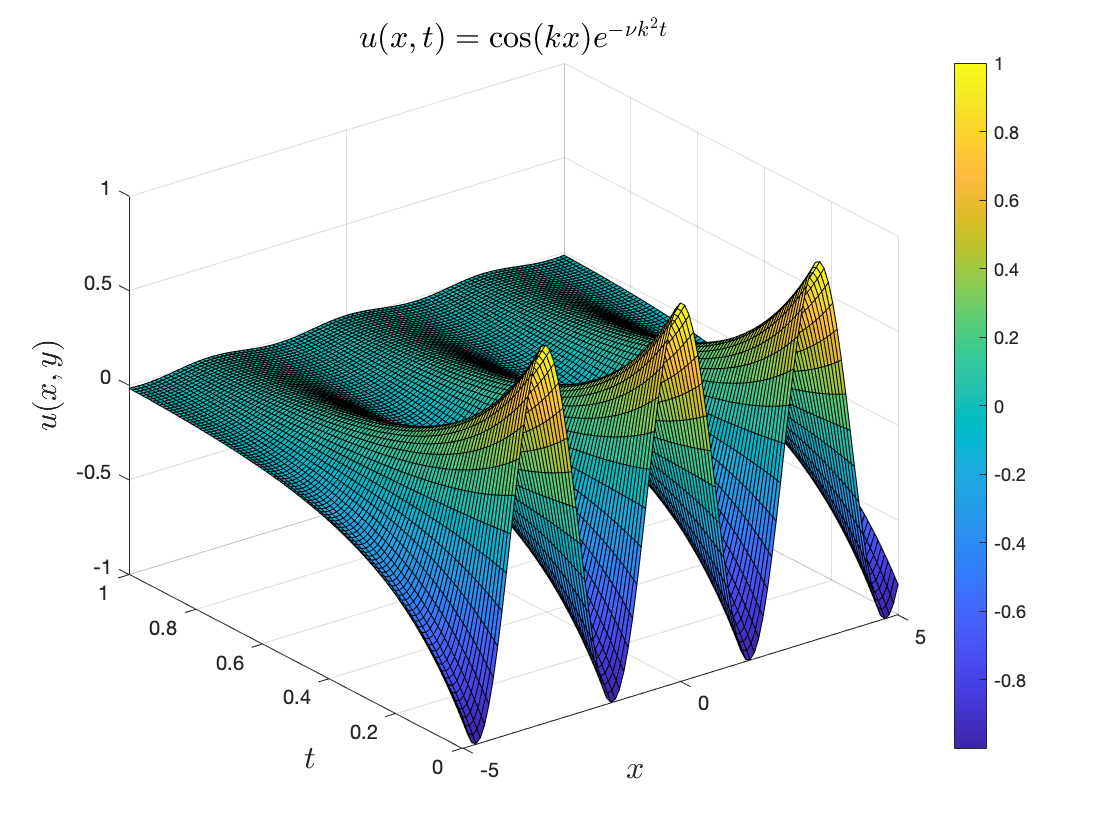
\includegraphics[width=5in]{q2b}
\caption{Plot of $u(x,t)$}
\label{fig:q2b}
\end{center}
\end{figure}

\item{\color{blue} \textit{Determine the exact solution to this with initial condition given by:}} $u(x,t=0) = H(x)$\\
The exact solution to the heat equation is given by: 
\begin{align*}
u(x,t) & = \frac{1}{\sqrt{4 \pi\nu t}}\int_{-\infty}^{\infty} H(\xi) \ e^{-(x-\xi)^2/4\nu t} \ d\xi \\
H(x) & = 
\begin{cases}
    1, & \text{if } x\geq 0\\
    0, & \text{otherwise}
\end{cases}
\end{align*}
So, 
\begin{align*}
u(x,t) = 
\begin{cases}
\frac{1}{\sqrt{4\pi\nu t}}\int_0^\infty e^{-(x-\xi)^2/4\nu t} \ d\xi &, x \geq 0 \\
0 &, \text{otherwise}
\end{cases}
\end{align*}
Let, $z = \frac{x-\xi}{\sqrt{4\nu t}}$
\begin{align*}
& \xi  \rightarrow 0 \Rightarrow z \rightarrow \frac{x}{\sqrt{4\nu t}} \\
& \xi  \rightarrow \infty \Rightarrow z \rightarrow -\infty \\
& \frac{-1}{\sqrt{4\nu t}}  = \frac{dz}{d\xi} \\
& \Rightarrow u(x,t) = -\frac{1}{\sqrt{\pi}}\int_\frac{x}{\sqrt{4\nu t}}^{-\infty} e^{-z^2} dz, \; \forall x\geq 0 \\
& \Rightarrow u(x,t) = \frac{1}{\sqrt{\pi}}\left[\int_{-\infty}^0 \ e^{-z^2} dz + \int_0^{\frac{x}{\sqrt{4\nu t}}} e^{-z^2} \ dz \ \right] \\
& e^{-z^2} \text{is a symmetric function and hence,} \\
& u(x,t) = \left[\frac{1}{2} + \frac{1}{2} \text{erf}\left(\frac{x}{\sqrt{4\nu t}}\right) \right] \; \forall \ x \geq 0 \\
\end{align*}
The surface plot is shown in Figure~\ref{fig:q2c}. The code for generating this plot is included in the Appendix. It can be seen that at time $t=0$, $u(x,t=0)$, clearly takes the shape of the Heavyside function $H(x)$. It is always 0 when $x<0$. Hence, this solution satisfies the initial condition as well as the PDE. 
\begin{figure}[t]
\begin{center}
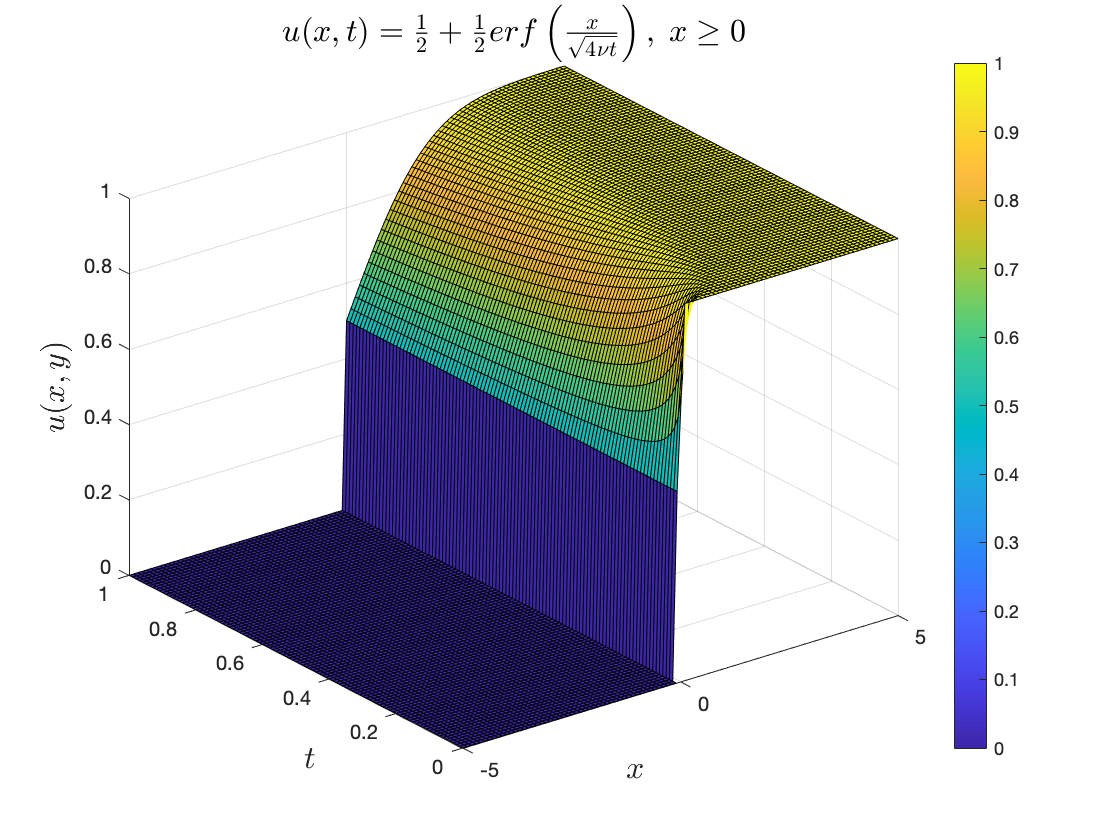
\includegraphics[width=5in]{q2c}
\caption{Plot of $u(x,t)$}
\label{fig:q2c}
\end{center}
\end{figure}

\end{enumerate}

\item{\color{red} PDE under consideration is:} $u_t = au_x + \nu u_{xx}$

\begin{enumerate}[label = (\alph*)]
\item{\color{blue} Determine the dispersion relationship for the PDE}\\
$A = \nu, B = 0, C = 0$ and $B^2 - AC = 0$. Hence this is a parabolic PDE. This can be transformed into the canonical form using a coordinate transformation.  Following the procedure outlined in Question 1.c), 
\begin{align*}
x & = \xi + c_1\eta \\
t & = c_2\xi + \eta \\
\xi & = \frac{1}{c_1c_2 - 1}(c_1t - x) \\
\eta & = \frac{1}{c_1c_2 - 1}(c_2x - t)\\
u_x & = u_\xi \ \xi_x + u_\eta \ \eta_x \\
u_{xx} & = u_{\xi\xi} \ \xi^2_x + u_{\eta\eta} \eta^2_x \; (\xi_{xx}, \eta_{xx} = 0 \; \text{because the relationship is linear})\\
u_t &= u_\xi \ \xi_t + u_\eta \ \eta_t 
\end{align*}
Substituting them into the PDE results in,
\begin{align*}
& \nu(\xi^2_x u_{\xi\xi} + \eta^2_x u_{\eta\eta}) + a(u_\xi \xi_x + u_\eta \eta_x) = u_\xi \xi_t + u_\eta \eta_t \\
& \text{Setting,} \; \nu \eta^2_x = 0 \Rightarrow c_2 = 0 \\
& \text{Setting,}\; a\xi_x -\xi_t = 0 \Rightarrow c_1 = -a \\
& \xi = x + at \\
& \eta = t 
\end{align*}
This coordinate transformation will result in converting the PDE into its canonical form:
\begin{align*}
\nu u_{\xi\xi} = u_\eta
\end{align*}
The dispersion relationship for this form is already derived in Q.2a) and its given by.
\begin{align*}
& u(\xi,\eta) = \hat{u}e^{ik\xi}e^{-i\omega \eta}\\
& \omega = -i\nu k^2 \\
& \text{Hence,} \; u(\xi,\eta) = \hat{u} e^{ik\xi}e^{-\nu k^2\eta} \\
& u(x,t) = \hat{u} e^{ik(x+at)}e^{-\nu k^2t}
\end{align*}

\item{\color{blue} Determine the exact solution to this with initial conditions:} $u(x,t=0) = \cos(kx)$ and, $a=1,\nu=1,k=2$.\\
Similar to the previous question, the solution is given by:
\begin{align*}
& u(x,t) = \cos(k(x+at))e^{-\nu k^2 t}\\
& u(x,t) = \cos(k(x+t))e^{-4t}
\end{align*}
The surface plot is shown in, Figure~\ref{fig: q3b}. This is similar to the result in Q.2b) with a transformed in the $x$ direction. 
\begin{figure}[htp]
\begin{center}
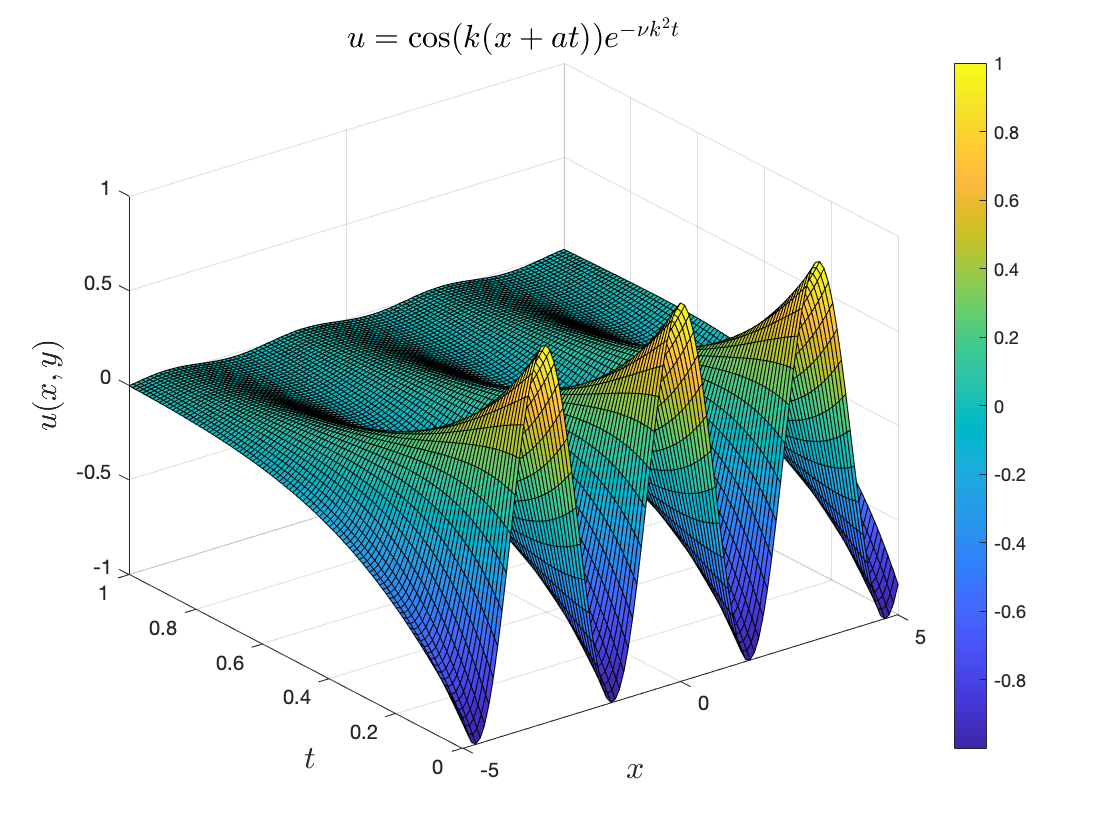
\includegraphics[width = 5in]{q3b}
\caption{Plot of $u(x,t)$}
\label{fig: q3b}
\end{center}
\end{figure}

\item{\color{blue}Determine the exact solution to this with initial conditions:} $u(x,t=0) = H(x)$ where, $H(x)$ is the Heavisde function. 
\begin{align*}
& u(\xi,\eta = 0) = H(\xi) \\
&  \Rightarrow u(\xi,\eta) = \frac{1}{2} + \frac{1}{2} \text{erf}\left(\frac{\xi}{\sqrt{4\nu \eta}}\right), \forall \xi \geq 0\\
& \text{Hence} \\
& u(x,t) = 
\begin{cases}
\frac{1}{2} + \frac{1}{2} \text{erf}\left(\frac{x+at}{\sqrt{4\nu t}}\right), & \text{if}\;  x+at \geq 0 \\
0 &, \text{otherwise}
\end{cases}
\end{align*} 
The surface plot is shown in, Figure~\ref{fig: q3c}. To show the change from the result in Q.2c) a contour plot that shows the transformation in the $x$ direction is provided in Figure~\ref{fig: q3c2}
\begin{figure}[htp]
\begin{center}
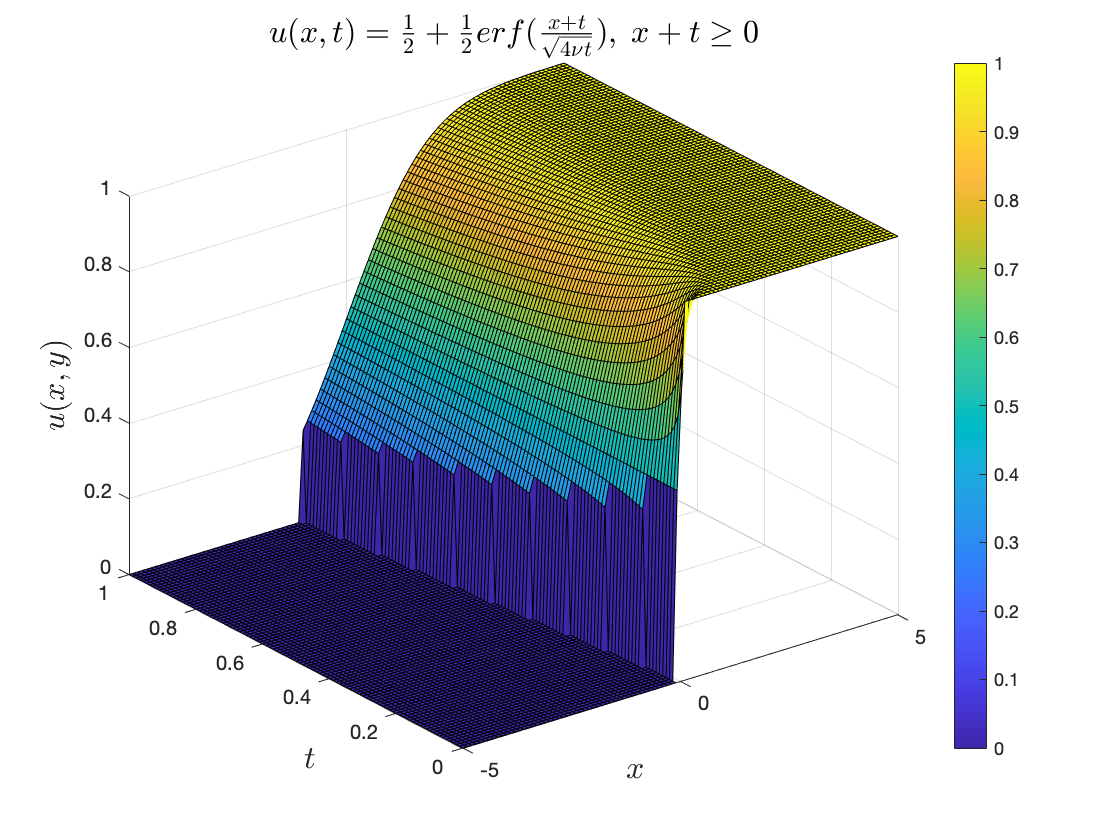
\includegraphics[width = 5in]{q3c}
\caption{Plot of $u(x,t)$}
\label{fig: q3c}
\end{center}
\end{figure}

\begin{figure}[htp]
\begin{center}
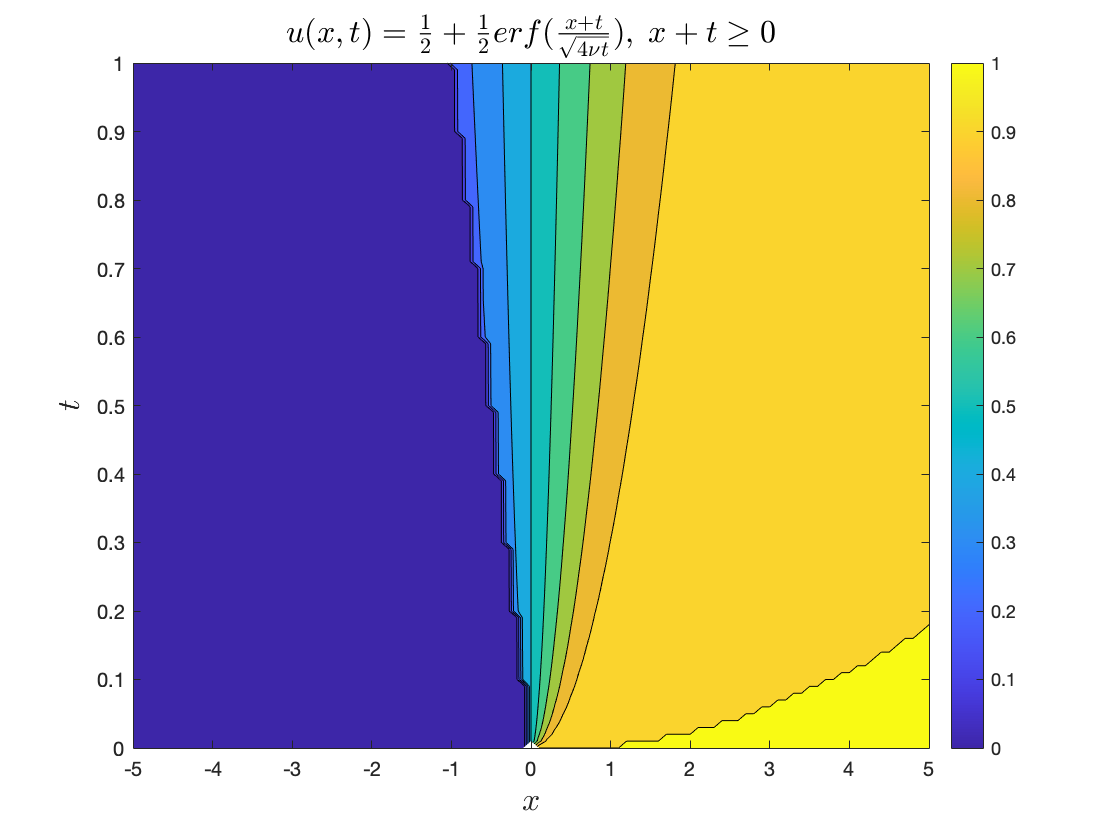
\includegraphics[width = 5in]{q3c2}
\caption{Plot of $u(x,t)$}
\label{fig: q3c2}
\end{center}
\end{figure}

\end{enumerate}

\item{\color{red} PDE under consideration is:} $u_{tt} = c^2 u_{xx} - 2a u_{tx}$ where $ c \in \mathbb{R}, a \in \mathbb{R}, x \in \mathbb{R}, t > 0$ 
\begin{enumerate}[label = (\alph*)]
\item{\color{blue} \textit{Determine the dispersion relation for this PDE.}}\\
Let $u = \hat{u}e^{ikx}e^{-i\omega t}$
\begin{align*}
u_t & = -i\omega \ u \\
u_{tt} & = (-i\omega)(-i\omega) \ u = \omega^2 \ u \\
u_x & = ik \ u\\
u_{xx} & = (ik) (ik) \ u = -k^2 \ u \\
u_{tx} & = \partial_x(u_t) = \partial_x(-i\omega \ u) = (-i\omega)(ik) \ u = k\omega \ u
\end{align*}
Substituting it in the PDE yields: 
\begin{align*}
\omega^2 \ u & = (c^2)(-k^2 \ u) - (2a)(k\omega \ u)\\
0 & = \omega^2 + 2ak\omega + c^2k^2 \\
\omega & = -a \pm \sqrt{a^2 - c^2k^2}
\end{align*}

\item{\color{blue} \textit{Determine the exact solution to this with initial conditions:}} $u(x,t=0) = \cos(kx)$, and, $u_t(x,t=0) = k(a+\sqrt{c^2 + a^2})\sin(kx)$ 
\begin{align*}
c^2u_{xx} -2au_{tx} - u_{tt} & = 0 \\
c^2u_{xx} -2au_{tx} + \frac{a^2}{c^2}u_{tt} - \frac{a^2}{c^2}u_{tt} -u_{tt} & = 0 \\
\left(c\partial_x - \frac{a}{c}\partial_t \right)^2u - \left(\left\{\sqrt{1 + \frac{a^2}{c^2}} \right\}\partial_t \right)^2u & = 0
\end{align*}
Now set: $\partial_\xi = c\partial_x - \frac{a}{c}\partial_t$ and, $\partial_\eta = \left(\left\{\sqrt{1 + \frac{a^2}{c^2}} \right\}\partial_t \right)$. This transforms the equation into its canonical form (wave equation): $u_{\xi\xi} - u_{\eta\eta} = 0$ \\
If a coordinate transformation is performed: 
\begin{align*}
\partial_\xi & = \partial_x \ x_\xi + \partial_t \ t_\xi \\
\partial_\eta & = \partial_x \ x_\eta + \partial_t \  t_\eta \\
\end{align*}

\begin{align*}
\begin{bmatrix}
\partial_\xi \\
\partial_\eta \\
\end{bmatrix} & = 
\begin{bmatrix}
c & -\frac{a}{c} \\ \\
0 & \sqrt{1 + \frac{a^2}{c^2}} \\
\end{bmatrix} 
\begin{bmatrix}
\partial_x \\
\partial_y
\end{bmatrix} \\
\begin{bmatrix}
\partial_\xi \\
\partial_\eta \\
\end{bmatrix} & = 
\begin{bmatrix}
x_\xi & t_\xi \\
x_\eta & t_\eta \\
\end{bmatrix}
\begin{bmatrix}
\partial_x \\
\partial_y
\end{bmatrix}
\end{align*}
This means, $x_\xi = c$, $t_\xi = -\frac{a}{c}$, $x_\eta = 0$, and, $t_\eta = \sqrt{1 + \frac{a^2}{c^2}}$. After integrating these equations, the following relations are obtained: 
\begin{align*}
x & = c\xi + c_1(\eta) \\
x_\eta & = 0 + \frac{dc_1}{d\eta} = 0 \Rightarrow c_1 = constant \\ \\
t & = -\frac{a}{c}\xi + c_2(\eta)\\
t_\eta & = 0 + \frac{dc_2}{d\eta} = \sqrt{1 + \frac{a^2}{c^2}} \Rightarrow c_2 = \sqrt{1 + \frac{a^2}{c^2}} \eta + constant \\
\end{align*}
Without loss of generality, the constants are set to $0$ and the transformed coordinate system is given by:
\begin{align*}
\xi & = \frac{x}{c} \\
\eta & = \frac{1}{\sqrt{1 + \frac{a^2}{c^2}}} \left\{ t + \frac{a}{c^2} x \right\} 
\end{align*}
The PDE has been transformed to $u_{\xi\xi} - u_{\eta\eta} = 0$ and the inverse relationship is given by: 
\begin{align*}
\begin{bmatrix}
\partial_x \\
\partial_t
\end{bmatrix}  = \frac{1}{c\sqrt{1 + \frac{a^2}{c^2}}} 
\begin{bmatrix}
\sqrt{1 + \frac{a^2}{c^2}} & \frac{a}{c} \\ \\
0 & c
\end{bmatrix} \begin{bmatrix}
\partial_\xi \\
\partial_\eta
\end{bmatrix}
\end{align*}
The determinant of this Jacobian is $|J| = 1 \neq 0$. Hence this is a non-singular transformation. Now if $t=0$, $\eta = \frac{a}{\sqrt{a^2 + c^2}}\xi$ and along this line, $u(\xi, \eta = m\xi) = \cos(kc\xi)$, where $m = \frac{a}{\sqrt{a^2 + c^2}}$. \\ \\
The second initial condition is, $u_t(x, t=0) = \frac{1}{\sqrt{1 + \frac{a^2}{c^2}}}u_\eta(\xi, \eta = m\xi) = k(a+\sqrt{a^2 + c^2}) \sin(kc\xi)$. Now, let $u_\eta(\xi, \eta = m\xi) = M\sin(kc\xi)$, where $M = \frac{k}{c}\sqrt{a^2 + c^2}(a + \sqrt{a^2 + c^2})$. \\ \\
The solution to this form of a wave equation is given by: 
\begin{align*}
u & = f(\xi - \eta) + g(\xi + \eta) \\
u_\eta & = -f'(\xi - \eta) + g'(\xi + \eta) 
\end{align*}
At $\eta = m\xi$, 
\begin{align}
u & = f((1-m)\xi) + g((1+m)\xi) = \cos(kc\xi) = \alpha(\xi)\\
u_\eta & = -f'((1-m)\xi) + g'((1+m)\xi) = M\sin(kc\xi) = \beta(\xi)
\end{align}
Integrating $(2)$ from $0 \rightarrow \xi$ results in the following equation: 
\begin{align}
\frac{-1}{1-m} f((1-m)\xi) + \frac{1}{1+m}g((1+m)\xi) = \int_0^\xi \beta(z) dz + c
\end{align}
Multiplying $(3)$ by $(1-m)$ and adding it to $(1)$ gives: 
\begin{align}
g((1+m)\xi) & = \frac{1+m}{2} \cos(kc\xi) + \frac{1-m^2}{2}\int_0^\xi \beta(z) dz + c \\
f((1-m)\xi) & = \frac{1-m}{2}\cos(kc\xi) - \frac{1-m^2}{2}\int_0^\xi \beta(z) dz - c
\end{align}
Change of variables $\xi \rightarrow \frac{\xi + \eta}{1+m}$ on $(4)$ and $\xi \rightarrow \frac{\xi - \eta}{1-m}$ on $(5)$ gives:
\begin{align*}
f(\xi - \eta) & = \frac{1-m}{2} \cos\left(\frac{kc}{1-m}(\xi-\eta)\right) - \frac{1-m^2}{2} \int_0^\frac{\xi - \eta}{1-m} \beta(z) dz - c \\
g(\xi + \eta) & = \frac{1+m}{2}\cos\left(\frac{kc}{1+m} (\xi + \eta)\right) + \frac{1-m^2}{2}\int_0^\frac{\xi + \eta}{1+m} \beta(z) dz + c \\
\end{align*}
Substituting $\beta(z) = M\sin(kcz)$ into the above expressions will give: 
\begin{align*}
u(\xi,\eta) & = \frac{1-m}{2}\cos\left(\frac{kc}{1-m}(\xi-\eta)\right) + \frac{1+m}{2}\cos\left(\frac{kc}{1+m}(\xi + \eta)\right) \\ & + \frac{M(1-m^2)}{2kc}\left[ \cos\left(\frac{kc}{1-m}(\xi-\eta)\right) - \cos\left(\frac{kc}{1+m}(\xi+\eta)\right) \right] \\
u(\xi,\eta) & = \cos\left(\frac{kc}{1-m}(\xi-\eta)\right)\left\{ \frac{1-m}{2} + \frac{M(1-m^2)}{2kc} \right\} + \\ & \cos\left(\frac{kc}{1+m}(\xi + \eta)\right) \left\{ \frac{1+m}{2} - \frac{M(1-m^2)}{2kc}\right\}
\end{align*}
Since $\xi = \xi(x,y)$ and, $\eta = \eta(x,y)$, plugging it in will result in:
\begin{align*}
u(x,t) & = \left\{ \frac{1-m}{2} + \frac{M(1-m^2)}{2kc}\right\} \cos\left(\frac{kc}{1-m} \left(\frac{1-m}{c}x - \frac{c}{\sqrt{a^2+c^2}}t \right)\right) + \\ & \left\{ \frac{1+m}{2} - \frac{M(1-m^2)}{2kc}\right\}\cos\left(\frac{kc}{1+m}\left(\frac{1+m}{c}x + \frac{c}{\sqrt{a^2+c^2}}t\right)\right)\\
\end{align*} 
It can be verified that this solution satisfies both the initial conditions $\forall x, t = 0$. The result has been plotted for $c=1, a=1, k=2$ on the following Figure~\ref{fig:q4b}. A wave-like behavior is observed and it propogates through time. This is an expected behavior given how its canonical form is a hyperbolic wave equation. The code to generate the plot has been attached in the Appendix. \\
\begin{figure}[htp]
  \begin{center}
  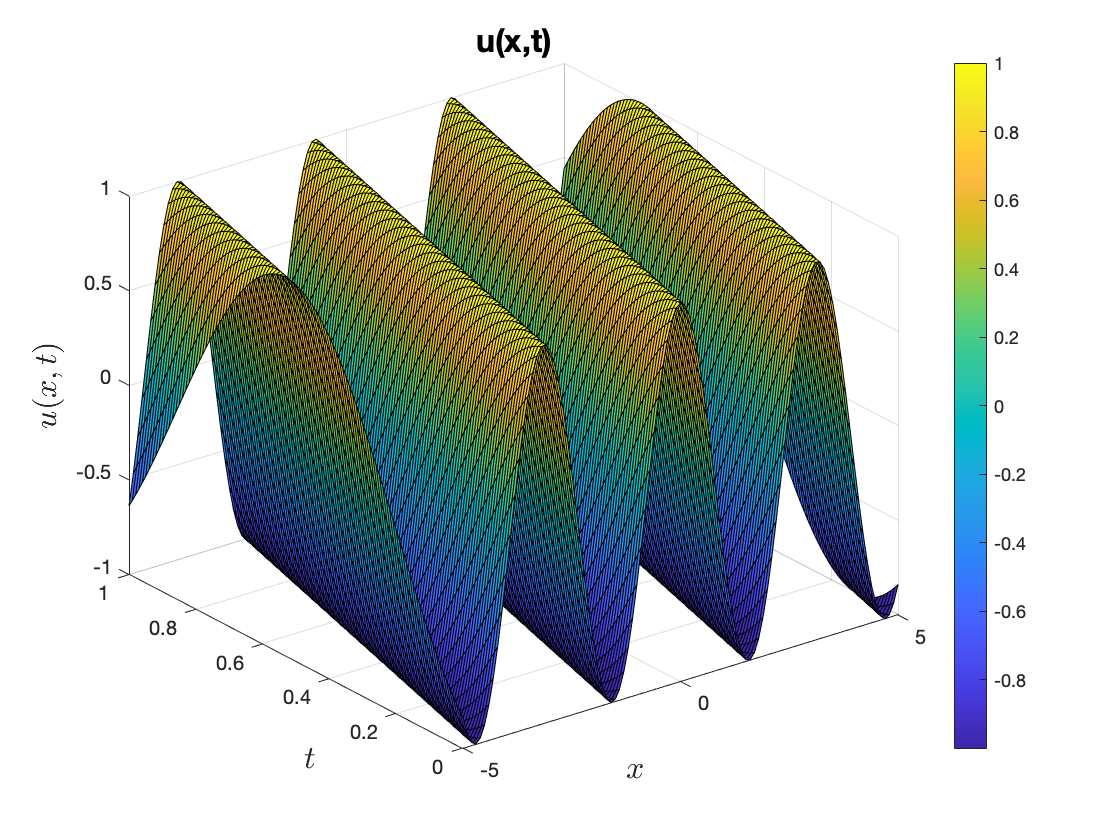
\includegraphics[width=5in]{q4b}
  \caption{Plot of $u(x,y)$.}
  \label{fig:q4b}
  \end{center}
\end{figure}

\item{\color{blue}\textit{Determine the exact solution subject to initial conditions:}} $u(x,t=0) = H(x)$ and, $u_t(x,t=0) = 1$. \\ \\
This equation can be converted to its canonical form $u_{\xi\xi} - u_{\eta\eta} = 0$ and the transformation was explained in part $(4.b)$.  It is given by:
\begin{align*}
\xi & = \frac{x}{c} \\ 
\eta & = \frac{c}{\sqrt{a^2 + c^2}}\left[t + \frac{a}{c^2} x\right]
\end{align*}
Application of this coordinate transformation leads to the initial conditions in the $\eta-\xi$ coordinate system: $u(\xi, \eta = m\xi) = H(c\xi)$ and, $u_t(x,t = 0) = \frac{c}{\sqrt{a^2+c^2}}u_\eta(\xi, \eta = m\xi) = 1$, where $m = \frac{a}{\sqrt{a^2 + c^2}}$. If $c \neq 0$
\begin{align*}
H(c\xi) = 
\begin{cases}
1, & c\xi \geq 0 \\
0, & c\xi < 0
\end{cases}
\end{align*}
The solution to this hyperbolic PDE is of the form: $u(\xi,\eta) = f(\xi-\eta) + g(\xi + \eta)$. At $\eta = m\xi$,
\begin{align}
f((1-m)\xi) + g((1+m)\xi) & = \alpha(\xi) = H(\xi) \\
-f'((1-m)\xi) + g'((1+m)\xi) & = \beta(\xi) = 1 
\end{align}
Integrating $(7)$ with respect to $\xi$ from $0 \rightarrow \xi$ yields:
\begin{align}
f((1-m)\xi) + g((1+m)\xi) & = \alpha(\xi) = H(\xi) \\
-\frac{1}{1-m}f((1-m)\xi) + \frac{1}{1+m}g((1+m)\xi) & = \int_0^\xi \beta(z) dz + c  
\end{align}
Solving for $f((1-m)\xi)$ and $g((1+m)\xi)$ and also applying change of variables $\xi \rightarrow \frac{\xi-\eta}{1-m}$  and $\xi \rightarrow \frac{\xi+\eta}{1+m}$ respectively yields, 
\begin{align*}
u(\xi,\eta) & = \frac{1-m}{2}H\left(\frac{\xi - \eta}{1-m}\right) + \frac{1+m}{2}H\left(\frac{\xi+\eta}{1+m}\right) + \eta - m\xi \\
u(x,t) & = \frac{1-m}{2} H\left(\frac{x}{c} - \frac{cm}{a(1-m)}t\right) + \frac{1+m}{2}H\left(\frac{x}{c} + \frac{cm}{a(1+m)}t\right) + \frac{cm}{a} t
\end{align*}
Here,
\begin{align*}
H\left(\frac{x}{c} - \frac{cm}{a(1-m)}t\right)  & = 
\begin{cases}
1, & \frac{x}{c} - \frac{cm}{a(1-m)}t \geq 0 \\
0, & \text{otherwise} 
\end{cases} \\
H\left(\frac{x}{c} + \frac{cm}{a(1+m)}t\right) & = 
\begin{cases}
1, & \frac{x}{c} + \frac{cm}{a(1+m)}t \geq 0 \\
0, & \text{otherwise}
\end{cases}
\end{align*}
The surface plot of the solution with $a = 1, c = 1$, is showin in Figure~\ref{fig:q4c}. The code to generate this plot is included in the Appendix. 
\begin{figure}[htp]
\begin{center}
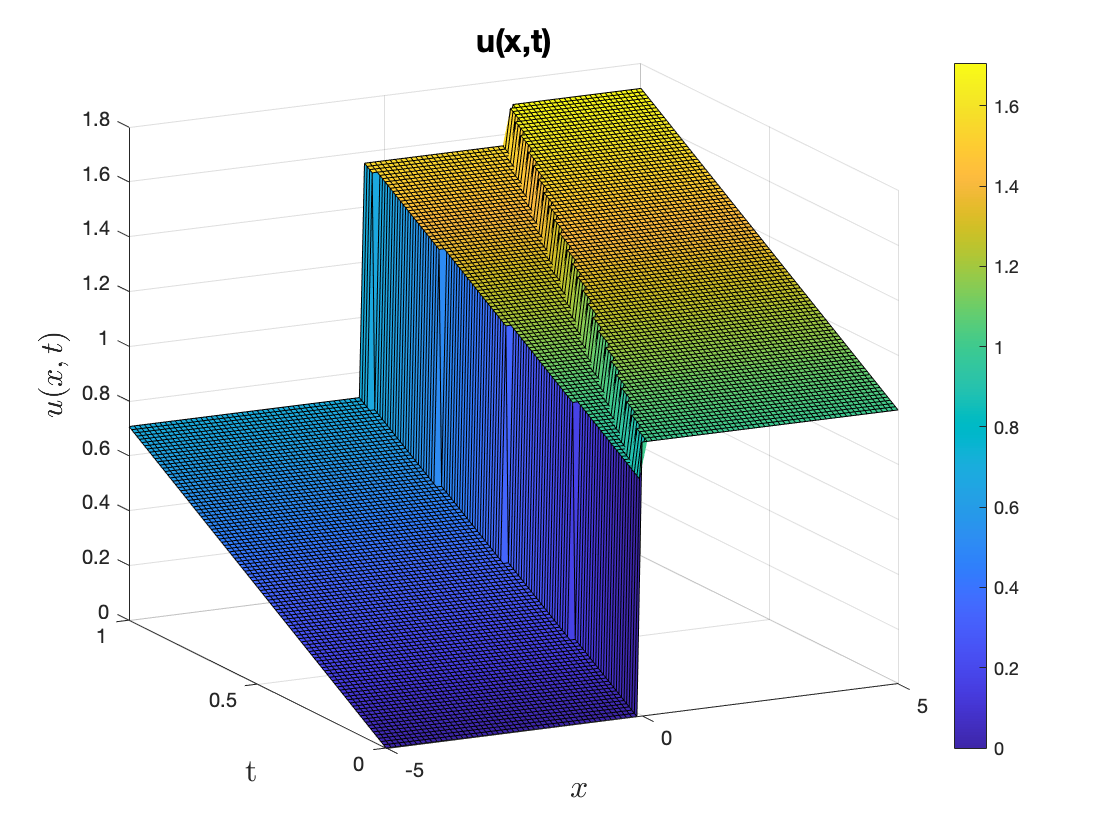
\includegraphics[width=5in]{q4c}
\caption{Plot of $u(x,t)$}
\label{fig:q4c}
\end{center}
\end{figure}
\end{enumerate}
There discontinuities in the solution because it is a linear combination of two Heaviside functions. It is a function with discontinuity. This solution also strongly satisfies the initial conditions imposed on the PDE. 
\end{enumerate}

\section{Appendix}
\lstinputlisting[language=Matlab, numbers=left, stepnumber=1, firstline=1,caption={Plotting code},label=code:myCode,frame=single]{HW1.m}

\end{document}